\chapter{Conception de l'intelligence artificielle}\label{chapter:intelligence-artificielle}

Pour la conception de l'intelligence artificielle, nous avons fait le choix de la variante nega-max de l'algorithme min-max
avec l'élagae alpha-béta.

Dans ce chapitre nous présentons nos fonctions d'évaluation de l'état du plateau (heuristiques),
puis nous rappelons ce qu'est min-max, nega-max et alpha-béta.

\section{Heuristiques}

Afin de permettre à l'I.A. de choisir quel coup jouer, plusieurs étapes sont nécessaires:
\begin{itemize}
    \item trouver l'ensemble des coups jouables
    \item évaluer les différents coups trouvés
    \item sélectionner et jouer le meilleur coup.
\end{itemize}

L'heuristique est utilisée à la deuxième étape, et sert à évaluer les différents coups possibles
— c'est à dire trouver si un coup est meilleur qu'un autre. Pour cela, l'heuristique analyse des
plateaux de jeu, où chaque plateau analysé représente l'état du jeu tel qu'il sera si l'I.A. joue
un coup en particulier. L'heuristique renvoie donc un nombre qui peut être faible (si le coup est
mauvais), ou élevé (si le coup est bon). La valeur calculée par l'heuristique nous sert alors à
évaluer la pertinence d'un coup. Nous avons développés différentes heuristiques, qui ont chacune
des performances différentes:

\subsection{L'heuristique facile: win-lose}

L'heuristique win-lose est l'heuristique la plus simple et est la première à avoir été implémentée.
Pour un plateau donné, elle renvoie la valeur maximum si l'I.A. a gagné, la valeur minimum si
l'I.A. a perdu, et 0 si aucun joueur n'a gagné. Cette méthode d'évaluation ne donne pas de très bon
résultats et n'est pas très bien élaguée par l'alpha-béta car elle ne s'intéresse qu'aux nœuds terminaux, tous les
autres sont équivalents.

\subsection{L'heuristique normale}

L'heuristique « normale » fonctionne de manière un peu plus subtile. Elle commence d'une manière similaire
à l'heuristique win-lose : le plateau est évalué à 100 si l'I.A. a gagné, et -100 si elle a perdu.
Dans le cas où la partie n'est pas terminée, cette heuristique va alors s'intéresser aux pions en place,
et va alors rajouter un point au plateau pour chaque pion de l'I.A. présent et chaque alignement de deux
pions de l'I.A., et procède de la même manière pour les pions du joueur adverse, en retranchant les points
au lieu de les ajouter. Avec cette heuristique, on obtient de bien meilleurs résultats qu'avec l'heuristique
de base, et une partie de Force 3 avec cette heuristique commence à devenir intéressante si la
profondeur n'est pas trop faibe.

\begin{figure}[H]
    \centering
    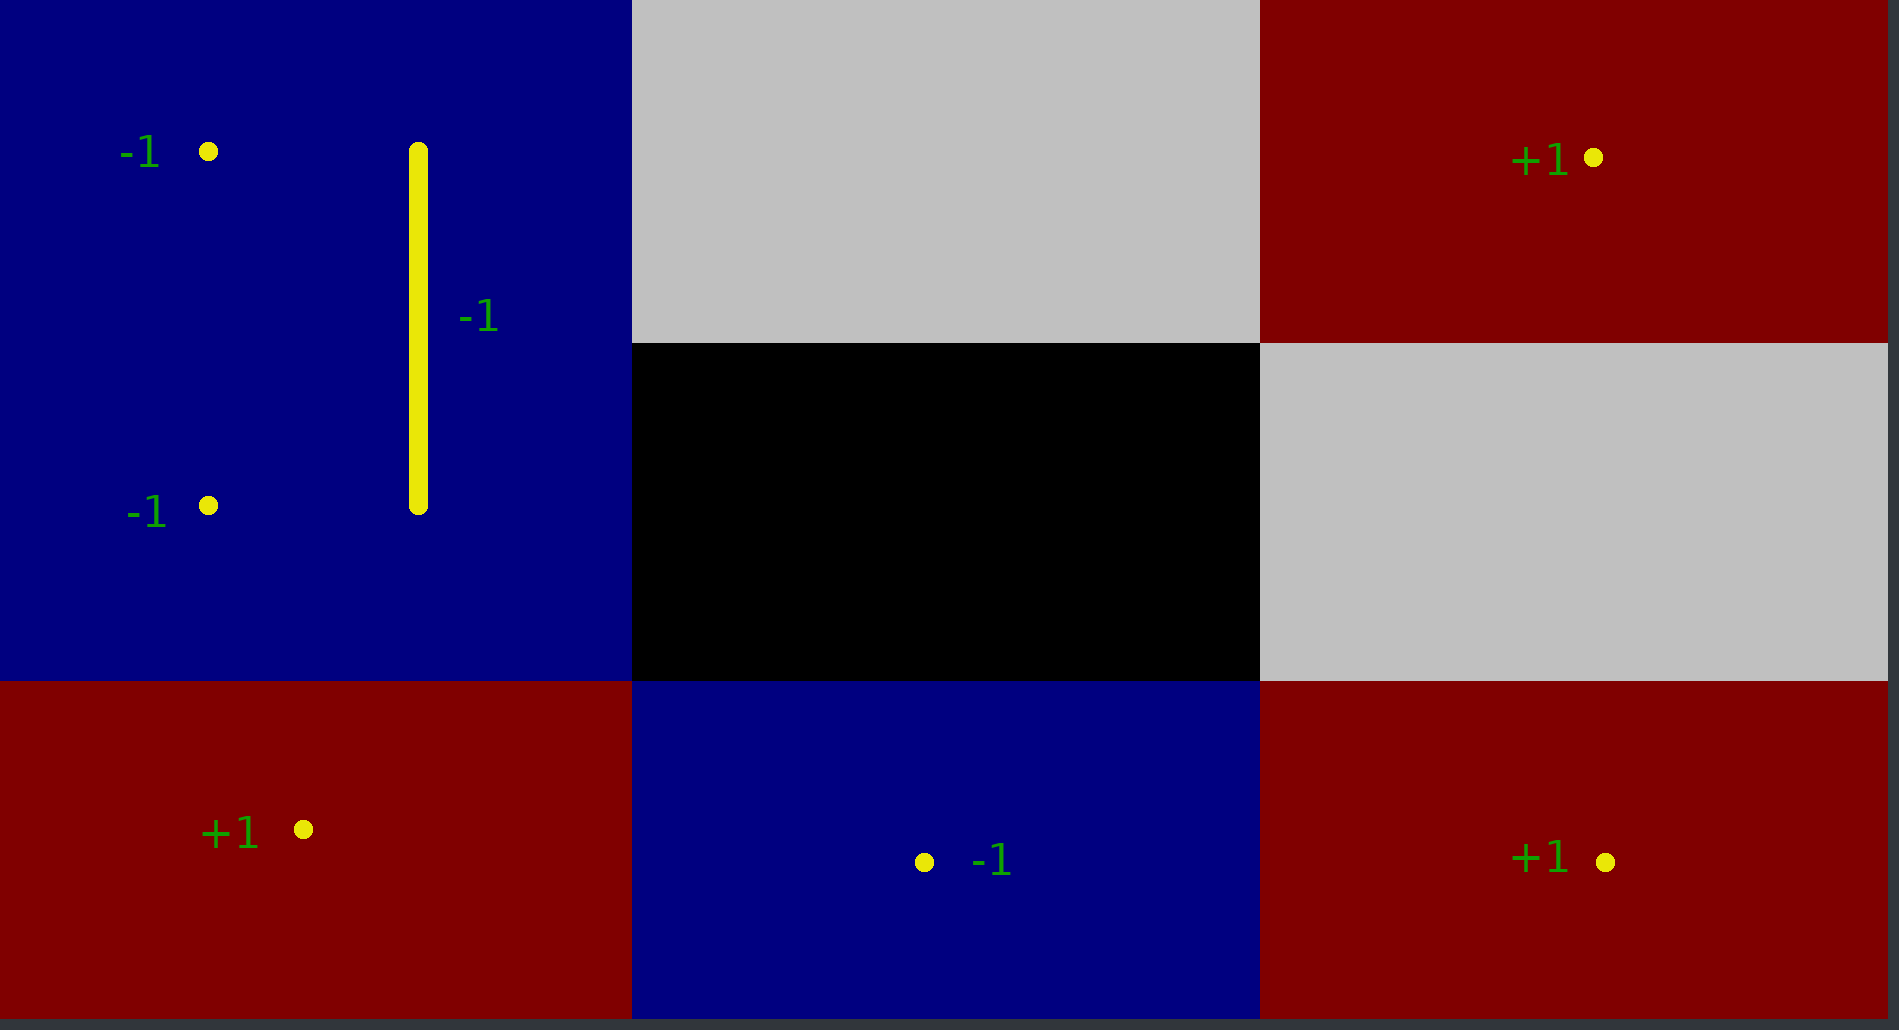
\includegraphics[width=0.8\textwidth]{Heuristic_Normal}{}
    \caption{exemple d'évaluation pour l'heuristique « normale », avec l'I.A. en rouge (évaluation: -1)}
\end{figure}

\subsection{L'heuristique difficile}

Cette heuristique fonctionne d'une manière similaire à l'heuristique « normale », mais en prenant plus de
cas en compte, notamment en ce qui concerne les alignements de deux pions (sur chaque lignes, colonnes et diagonales):

\begin{table}[H]
    \begin{tabular}{lc}
        Un pion allié                                 & +5    \\
        Deux pions alliés et un pion adverse          & +11   \\
        Deux pions alliés et une case vide (noire)    & +16   \\
        Deux pions alliés et une case libre (blanche) & +21   \\
        Trois pions alliés                            & +1000 \\
    \end{tabular}
    \caption{Poids des différentes combinaisons de pions}
\end{table}

Les mêmes valeurs, évaluées pour l'adversaire, sont soustraites.

\begin{figure}[H]
    \centering
    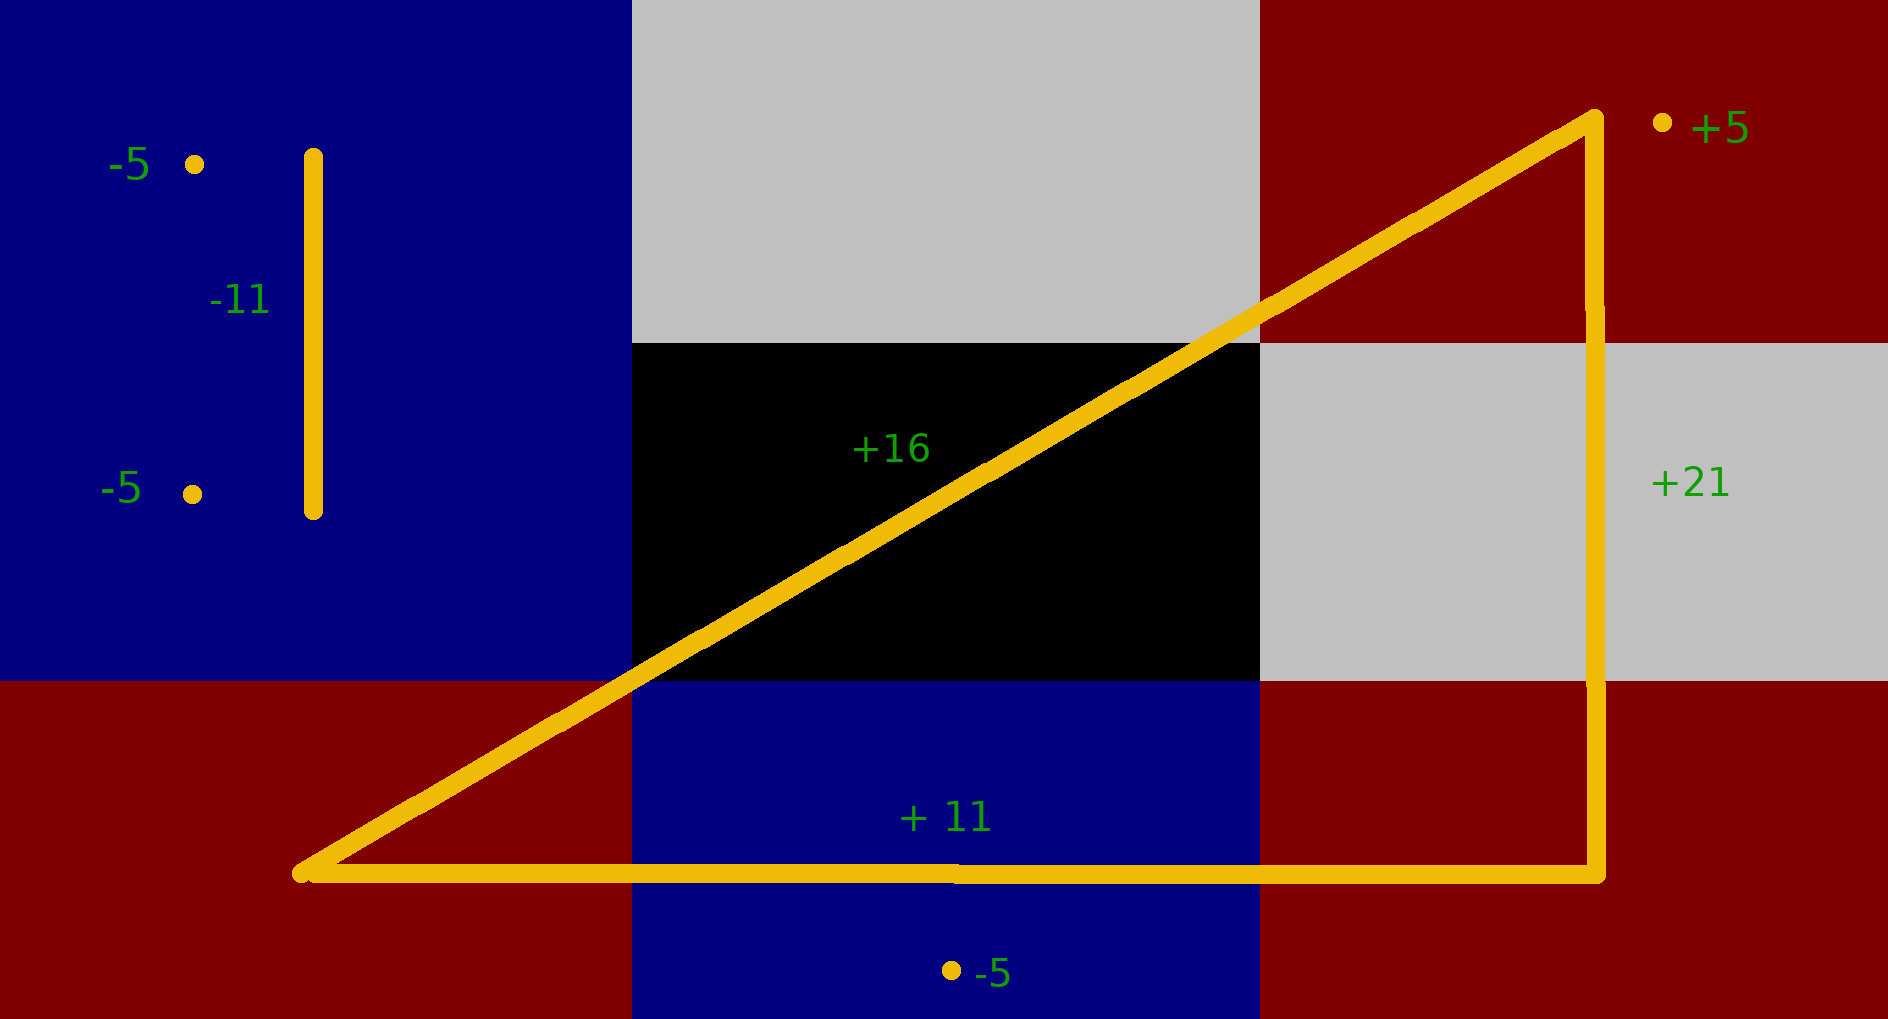
\includegraphics[width=0.8\textwidth]{Heuristic_Hard}{}
    \caption{exemple d'évaluation d'un plateau avec l'heuristique « difficile », avec l'I.A. en rouge (évaluation: +27)}
\end{figure}

L'extrait de code pour cette heuristique se trouve à l'annexe \ref{src:heuristic_hard}.

\subsection{Légendaire}

L'heuristique « légendaire » est une amélioration de l'heuristique « difficile ». Elle commence tout d'abord par évaluer
le plateau de la même manière que celle-ci, mais s'intéresse ensuite à l'emplacement de la case vide (noire). En effet,
de part sa mobilité, celle-ci permet des alignements de trois « indirects », et mérite donc un traitement particulier.

\begin{figure}[H]
    \centering
    
\includegraphics[width=0.8\textwidth]{Heuristic_Legendary}{}
    \caption{exemple d'évaluation un morceau de plateau avec l'heuristique « légendaire », avec l'I.A. en rouge (évaluation: +141, contre +26 pour l'heuristique précédente)}
\end{figure}

Les heuristiques se trouvent dans le fichier \emph{src/logic/heuristic.cpp}.

\section{Rappel de l'algorithme du min-max}

Le min-max est un algorithme visant à minimiser la perte maximum dans le cas d'un jeu à somme nulle
et informations complètes pour deux joueurs. On cherche donc à
maximiser son gain tandis que l'adversaire cherche à le minimiser (autrement dit à maximiser le
sien étant donné que le jeu est à somme nulle).
Le principe de l'algorithme est très simple : on parcourt l'arbre de jeu dans le but de faire remonter
à la racine un score qui est associé à la meilleure transition estimée.
Pour cela, on doit distinguer deux types de nœuds : les nœuds max (nœuds joueur) et les nœuds min (nœuds adverse).
Les nœuds min prennent la valeur la plus faible de leurs enfants tandis que les nœuds max prennent la valeur la
plus élevée de leurs enfants.
Pour les feuilles de l'arbre, on évalue l'état correspondant du jeu avec l'une des heuristiques précédentes.

Voici un arbre d'exemple :

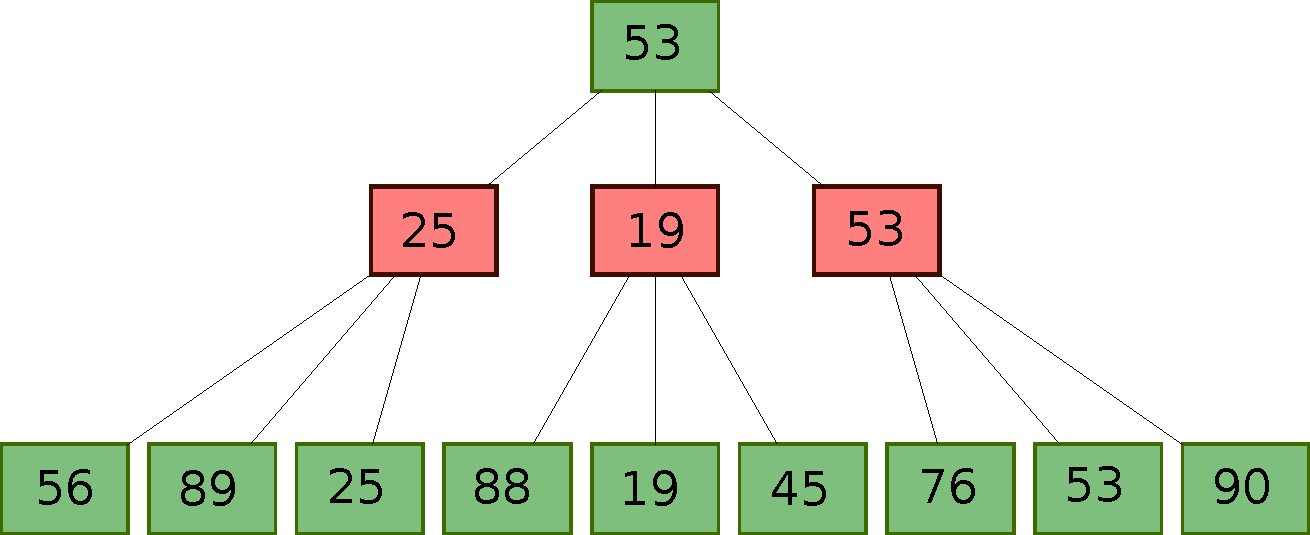
\includegraphics[scale=0.6]{minmax}

Les nœuds verts sont ici des nœuds max et les nœuds rouges des nœuds min.

On voit ici que la transition à choisir est la troisième qui assure d'obtenir un gain de 53 dans le pire des cas.
Même s'il est possible de gagner plus dans d'autres cas, on part du principe que l'adversaire ne nous laissera pas faire.

\section{Nega-max sans élagage}

Il existe une simplification du min-max, le principe restant rigoureusement le même.
L'idée est simplement de toujours prendre l'opposé des valeurs enfants.
En effet : prendre le maximum de l'opposé des valeurs est équivalent à prendre le minimum des valeurs.
Ainsi, il n'est plus nécessaire de gérer trois cas (feuille, min, max), mais seulement deux (feuille, max).

Exemple sur l'arbre précédent :

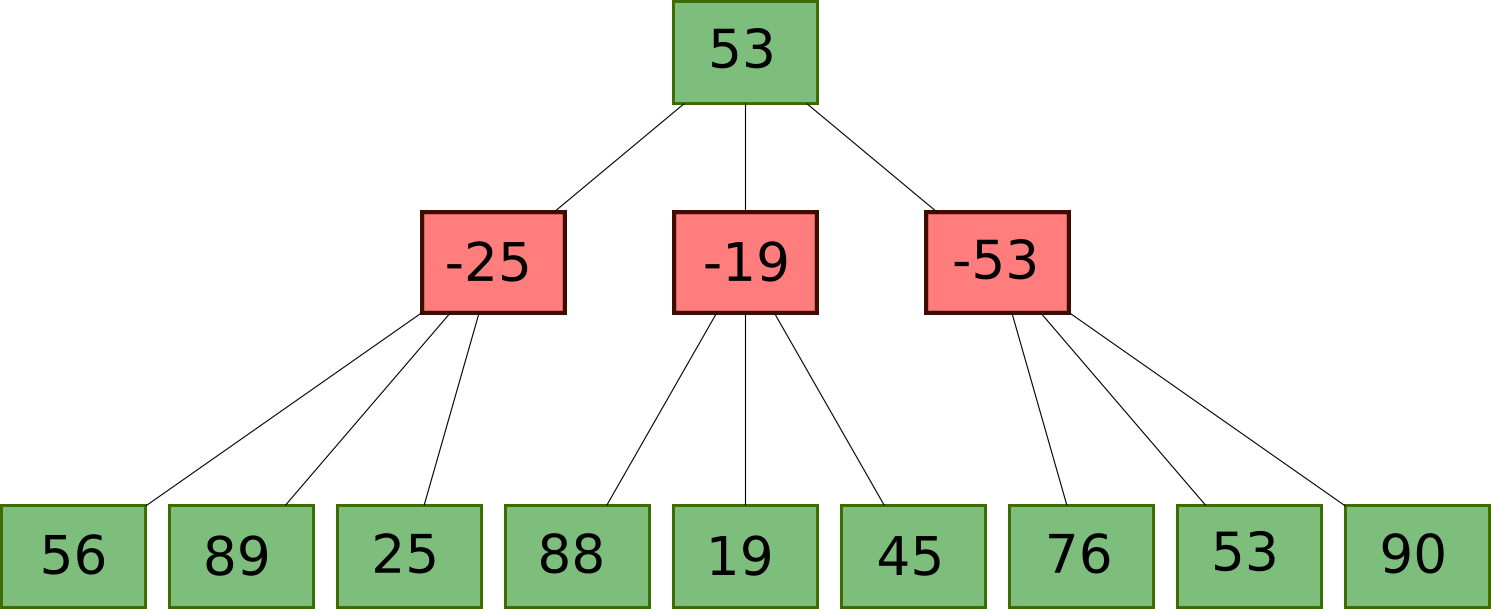
\includegraphics[scale=0.6]{negamax}

Les résultats sont identiques.

\section{Nega-max avec élagage alpha-béta}

Les algorithmes précédents effectuent une exploration complète de l'arbre alors qu'il est possible de n'effectuer
qu'une exploration partielle de l'arbre en élagant les transitions dont on est sûr que la qualité des solutions générées
sera inférieure ou égale.

Le principe de l'élagage alpha-béta est de garder la trace d'une borne inférieure (\(\alpha\)) et supérieure (\(\beta\))
pour chaque nœud. Lorsque la borne inférieure est supérieure à la borne supérieure, on arrête l'exploration des nœuds frères.
On met à jour la borne inférieure sur les nœuds max et la borne supérieure sur les nœuds min.

Exemple :

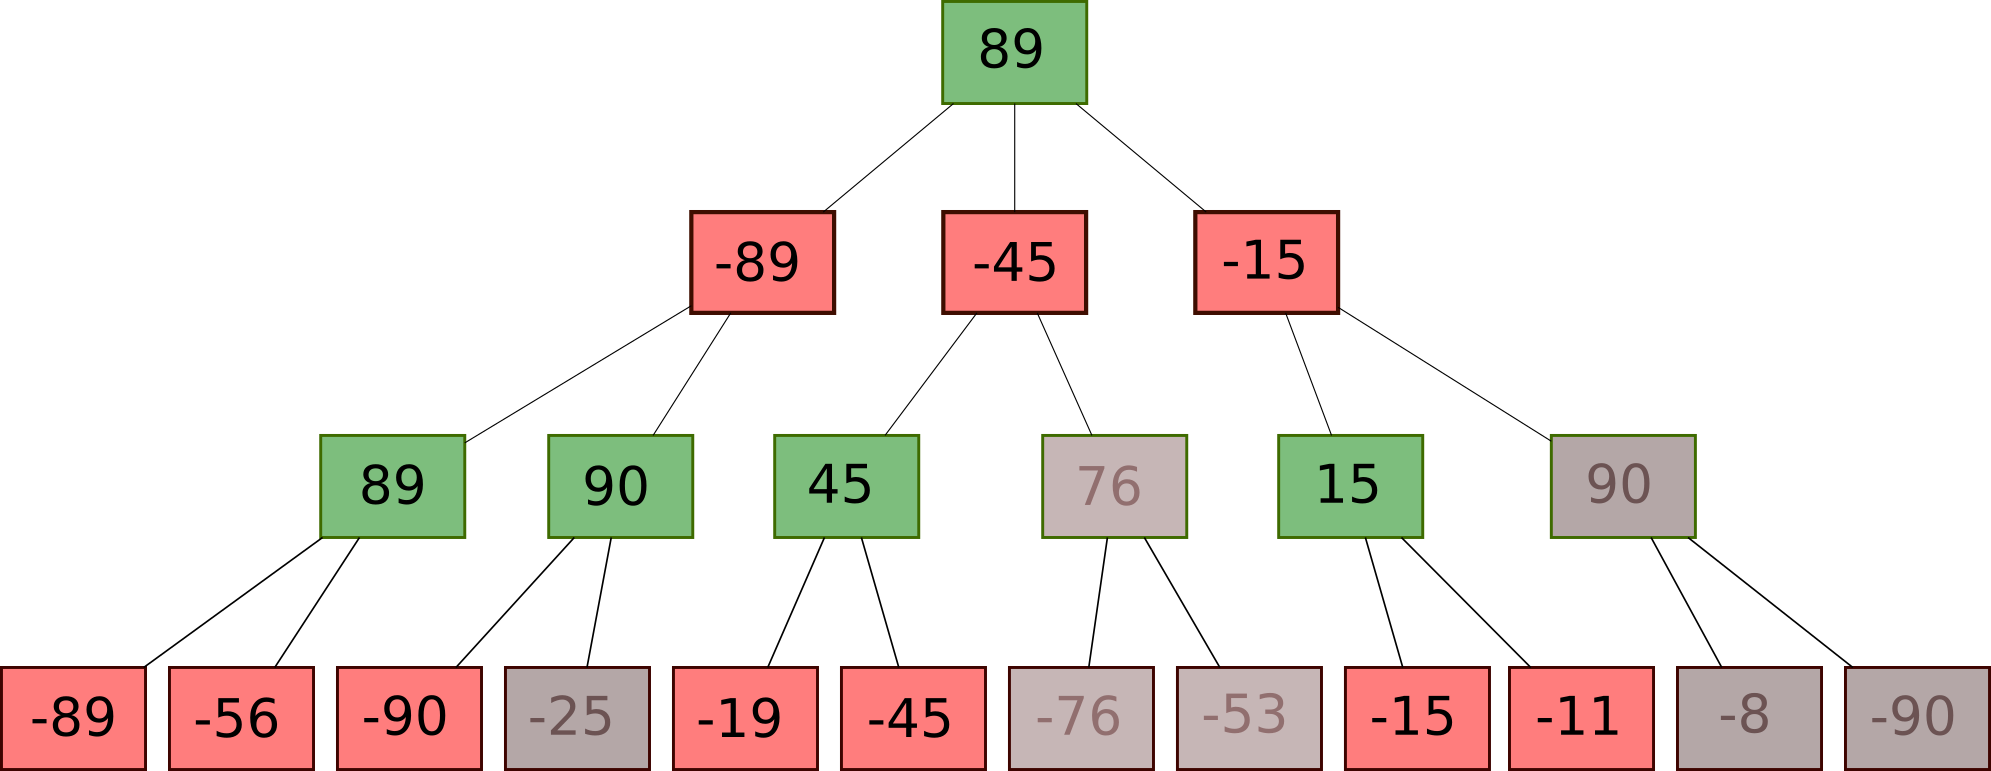
\includegraphics[scale=0.5]{negamax-alphabeta}

Ici, on effectue trois coupures :
\begin{itemize}
    \item le nœud max a été mis à jour à 90 (\(\alpha\) = 90). Comme c'est un nœud max, il ne peut qu'augmenter.
        La valeur de \(\beta\) est à 89. On effectue donc la coupure (\(\alpha > \beta\)).
    \item le nœud min a été mis à jour à 45 (\(\beta\) = 45). Comme c'est un nœud min, il ne peut que diminuer.
        La valeur de \(\alpha\) est à 89. On effectue donc la coupure.
    \item le nœud min a été mis à jour à 15 (\(\beta\) = 15). Comme c'est un nœud min, il ne peut que diminuer.
        La valeur de \(\alpha\) est à 89. On effectue donc la coupure.
\end{itemize}

L'extrait de code du nega-max avec élagage alpha-béta se trouve à l'annexe \ref{src:negamax}.

\section{Amélioration de la prise de décision}

Nous avons également ajouté quelques fonctionnalités dans notre implémentation du nega-max :

\begin{itemize}
    \item L'IA peut choisir aléatoirement une transition parmi toutes celles qui ont obtenu un score identique.
    \item L'élagage alpha-béta n'est activé que lorsque l'on demande une profondeur supérieure à un certain seuil fixé.
        En effet, lorsque la profondeur n'est pas trop élevé, l'absence d'élagage ne pose aucun problème de performances et
        permet de déterminer plus de transitions équivalentes et donc de permettre de diversifier le jeu de l'IA : plus
        intéressant en tant que joueur.
    \item On ajoute [la profondeur actuelle \(-\) la profondeur maximale] au score des nœuds terminaux pour priviligier les
        transitions qui mènent à une victoire plus rapide. Seuls les nœuds terminaux qui entraînent la défaite ou la victoire
        n'ont pas toujours la profondeur actuelle égale à la profondeur maximale et sont donc les seuls concernés par cette
        amélioration. Ainsi, l'IA ne cherchera jamais à faire durer inutilement la partie que ce soit parce qu'elle a gagné
        d'avance ou perdu d'avance.
\end{itemize}

L'extrait de code pour la prise de décision se trouve à l'annexe \ref{src:think}.

